\documentclass[11pt,a4paper]{report}

\usepackage[utf8]{inputenc}
\usepackage[T1]{fontenc}
\usepackage{lmodern}
\usepackage[margin=1in]{geometry}
\usepackage{graphicx}
\usepackage{xcolor}
\usepackage{listings}
\usepackage{hyperref}
\usepackage{booktabs}
\usepackage{enumitem}
\usepackage{fancyhdr}
\usepackage{titlesec}
\usepackage{tocloft}
\usepackage{amsmath}
\usepackage{algorithm}
\usepackage{algpseudocode}
\usepackage{tikz}
\usetikzlibrary{shapes.geometric, arrows.meta, positioning, calc}

% Colors
\definecolor{codebackground}{RGB}{245,245,245}
\definecolor{codecomment}{RGB}{0,128,0}
\definecolor{codekeyword}{RGB}{0,0,180}
\definecolor{codestring}{RGB}{163,21,21}
\definecolor{linkcolor}{RGB}{0,80,160}
\definecolor{chaptercolor}{RGB}{40,60,100}
\definecolor{squaredark}{RGB}{181,136,99}
\definecolor{squarelight}{RGB}{240,217,181}

% Hyperref setup
\hypersetup{
    colorlinks=true,
    linkcolor=linkcolor,
    urlcolor=linkcolor,
    citecolor=linkcolor,
    pdftitle={Kirin Board Interpreter Documentation},
    pdfauthor={Strydr Silverberg},
}

% Code listing style
\lstdefinestyle{codestyle}{
    backgroundcolor=\color{codebackground},
    basicstyle=\ttfamily\small,
    breakatwhitespace=false,
    breaklines=true,
    captionpos=b,
    commentstyle=\color{codecomment}\itshape,
    keywordstyle=\color{codekeyword}\bfseries,
    stringstyle=\color{codestring},
    numberstyle=\tiny\color{gray},
    numbers=left,
    numbersep=8pt,
    showspaces=false,
    showstringspaces=false,
    showtabs=false,
    tabsize=4,
    frame=single,
    framerule=0.5pt,
    rulecolor=\color{gray!50},
}
\lstset{style=codestyle}

% Chapter and section styling
\titleformat{\chapter}[display]
    {\normalfont\huge\bfseries\color{chaptercolor}}
    {\chaptertitlename\ \thechapter}{20pt}{\Huge}
\titlespacing*{\chapter}{0pt}{0pt}{30pt}

% Header and footer
\pagestyle{fancy}
\fancyhf{}
\fancyhead[L]{\leftmark}
\fancyhead[R]{\thepage}
\setlength{\headheight}{14pt}
\renewcommand{\headrulewidth}{0.4pt}

% Function/method documentation macro
\newcommand{\function}[4]{%
    \paragraph{\texttt{#1}} \hfill \textit{#2}\\
    \textbf{Parameters:} #3\\
    \textbf{Returns:} #4
}

% Note box
\newcommand{\notebox}[1]{%
    \begin{center}
    \fcolorbox{gray}{gray!10}{%
        \parbox{0.9\textwidth}{\textbf{Note:} #1}
    }
    \end{center}
}

% Warning box
\newcommand{\warningbox}[1]{%
    \begin{center}
    \fcolorbox{red!70}{red!10}{%
        \parbox{0.9\textwidth}{\textbf{Warning:} #1}
    }
    \end{center}
}

%------------------------------------------------------------------------------
% Document Information
%------------------------------------------------------------------------------
\title{%
    \vspace{-1cm}
    \rule{\textwidth}{1pt}\\[0.5cm]
    {\Huge\bfseries Kirin}\\[0.3cm]
    {\Large Board Interpreter Documentation}\\[0.3cm]
    \rule{\textwidth}{1pt}\\[1cm]
    {\large Current Repository Build}
}
\author{Strydr Silverberg\\strydr\_silverberg@mines.edu\\\\Colorado School of Mines}
\date{\today}

\begin{document}

\maketitle
\thispagestyle{empty}

\vfill
\begin{center}
    \textit{Board Interpreter: Physical move planning and path generation for the Kirin autonomous chess system}\\[1em]
    \textbf{2026 Colorado School of Mines ProtoFund Recipient}\\
    Team: Strydr Silverberg, Colin Dake
\end{center}
\vfill

\newpage
\tableofcontents
\newpage

%==============================================================================
\chapter{Introduction}
%==============================================================================

\section{Overview}

This document provides comprehensive documentation for the \textbf{Board Interpreter} module of the Kirin autonomous chess system. The board interpreter is the translation layer between the abstract chess world of the Kirin engine and the physical reality of the robotic gantry that moves pieces on the board.

When the Kirin engine decides on a move, it communicates that decision as a UCI move string (e.g., \texttt{e2e4}). The board interpreter's job is to answer the question: \emph{how does the robot actually execute that move on a physical board with pieces that may be in the way?} This involves computing geometrically valid physical paths for the magnetic gantry head, detecting pieces that block those paths, temporarily relocating blockers to safe parking squares, and finally generating a complete ordered action plan for the gantry controller to execute step by step.

\section{Responsibilities}

The board interpreter module is responsible for:

\begin{itemize}
    \item \textbf{Coordinate translation}: Converting between FEN algebraic notation and physical \texttt{(row, col)} grid coordinates.
    \item \textbf{Physical board state tracking}: Maintaining a temporary occupancy model of the board during move planning so that blocker relocations can be simulated before being sent to the gantry.
    \item \textbf{Piece-type-aware path generation}: Computing one or more geometrically valid sweep paths for each piece type (pawns, knights, bishops, rooks, queens, and kings), reflecting how the gantry head must physically travel.
    \item \textbf{Blocker detection and relocation planning}: Identifying pieces that obstruct the chosen path and computing sub-plans to park them temporarily on safe empty squares.
    \item \textbf{A* pathfinding for blocker routing}: Finding collision-free routes for blocker pieces being moved to and from parking spots, using A* search with Chebyshev distance as the heuristic.
    \item \textbf{Move plan assembly}: Packaging the complete sequence of relocations, the primary piece move, and post-move restorations of parked pieces into a \texttt{MovePlan} structure that the gantry controller can execute directly.
\end{itemize}

\section{Position in the System Architecture}

The board interpreter sits between the chess engine and the gantry controller in the Kirin software stack:

\begin{center}
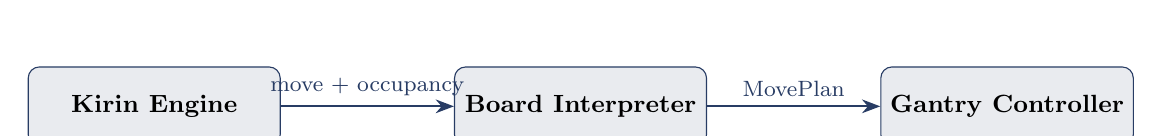
\begin{tikzpicture}[
    box/.style={rectangle, draw=chaptercolor, fill=chaptercolor!10, rounded corners=4pt,
                minimum width=3.2cm, minimum height=1.0cm, text centered, font=\small\bfseries},
    arrow/.style={-Stealth, thick, color=chaptercolor}
]
    \node[box] (engine)  {Kirin Engine};
    \node[box, right=2.2cm of engine] (interp) {Board Interpreter};
    \node[box, right=2.2cm of interp] (gantry) {Gantry Controller};

    \draw[arrow] (engine)  -- node[above, font=\footnotesize]{move + occupancy} (interp);
    \draw[arrow] (interp)  -- node[above, font=\footnotesize]{MovePlan} (gantry);
\end{tikzpicture}
\end{center}

The engine provides two pieces of information: the move in UCI notation and a bitboard encoding which squares are currently occupied. The board interpreter uses these to produce a fully sequenced \texttt{MovePlan}. The gantry controller then executes each step of that plan in order without needing to reason about board geometry.

\section{Coordinate System}

The board interpreter uses a \texttt{(row, col)} coordinate system that maps directly to the physical grid layout of the board:

\begin{table}[h]
\centering
\begin{tabular}{lll}
\toprule
\textbf{Axis} & \textbf{Range} & \textbf{Convention} \\
\midrule
Row & 0--7 & Row 0 = rank 8 (far side from white), Row 7 = rank 1 \\
Col & 0--7 & Col 0 = file a (left side), Col 7 = file h (right side) \\
\bottomrule
\end{tabular}
\caption{Physical board coordinate conventions}
\end{table}

Square indices used in the underlying bitboard follow the engine convention: bit 0 corresponds to \texttt{a8} (row 0, col 0) and bit 63 corresponds to \texttt{h1} (row 7, col 7). The formula is \texttt{square = row * 8 + col}.

%==============================================================================
\chapter{Data Structures}
%==============================================================================

\section{BoardCoord}

\texttt{BoardCoord} is the fundamental coordinate type used throughout the module. It represents a single square on the physical board.

\begin{lstlisting}[language=C++, caption={BoardCoord definition}]
struct BoardCoord {
    int row;
    int col;

    BoardCoord();
    BoardCoord(int r, int c);

    bool operator==(const BoardCoord& other) const;
    bool operator!=(const BoardCoord& other) const;
    bool operator<(const BoardCoord& other) const;

    int toSquareIndex() const;
    static BoardCoord fromSquareIndex(int square);
    static BoardCoord fromFEN(const char* str);
    void toFEN(char* out) const;
};
\end{lstlisting}

\subsection{Member Functions}

\function{toSquareIndex() const}{Method}{None}{int -- square index in range [0, 63]}

Converts the \texttt{(row, col)} coordinate to a linear square index using the formula \texttt{row * 8 + col}. This index is compatible with the bitboard representation used by the Kirin engine.

\function{fromSquareIndex(int square)}{Static Method}{square -- linear index [0, 63]}{BoardCoord}

Constructs a \texttt{BoardCoord} from a square index. Inverse of \texttt{toSquareIndex}.

\function{fromFEN(const char* str)}{Static Method}{str -- two-character FEN string, e.g. \texttt{"e4"}}{BoardCoord}

Parses a FEN algebraic square name into physical \texttt{(row, col)} coordinates. The file character (\texttt{a}--\texttt{h}) maps to column 0--7 and the rank digit (\texttt{1}--\texttt{8}) is flipped to row 7--0 respectively. Returns \texttt{BoardCoord(0,0)} on invalid input.

\function{toFEN(char* out) const}{Method}{out -- output buffer of at least 3 bytes}{void}

Serialises the coordinate back to a two-character FEN algebraic string followed by a null terminator. Inverse of \texttt{fromFEN}.

\subsection{Ordering}

The \texttt{operator<} overload allows \texttt{BoardCoord} values to be stored in \texttt{std::set} and \texttt{std::map} containers. Ordering is row-major: coordinates are compared first by row, then by column.

\section{Path}

A \texttt{Path} is an ordered sequence of squares that the gantry head must visit while carrying a piece. The first element is the first square entered \emph{after} the starting position, and the last element is the destination square.

\begin{lstlisting}[language=C++, caption={Path definition}]
struct Path {
    std::vector<BoardCoord> squares;

    void append(const BoardCoord& coord);
    void clear();
    int length() const;
    bool empty() const;
    BoardCoord destination() const;
};
\end{lstlisting}

\notebox{Paths do not include the source square. They contain every intermediate square the gantry crosses plus the final destination, making the length equal to the number of squares traversed (not the chess-move distance).}

\section{PieceType}

An enum identifying the type of piece involved in a move. The board interpreter uses this to select the appropriate path generation algorithm.

\begin{lstlisting}[language=C++, caption={PieceType enum}]
enum PieceType {
    PAWN, KNIGHT, BISHOP, ROOK, QUEEN, KING, UNKNOWN
};
\end{lstlisting}

When \texttt{PieceType} is \texttt{UNKNOWN}, the path generator falls back to inferring the movement style from the geometric relationship between source and destination squares.

\section{PhysicalMove}

Encapsulates a single physical piece movement: where a piece starts, where it ends, what type it is, and whether the move is a capture.

\begin{lstlisting}[language=C++, caption={PhysicalMove definition}]
struct PhysicalMove {
    BoardCoord from;
    BoardCoord to;
    PieceType  pieceType;
    bool       isCapture;
};
\end{lstlisting}

\section{RelocationPlan}

Represents the plan to temporarily move a single blocking piece out of the way of a primary piece move. It records both the source and destination parking square, and the A*-computed path the gantry will follow.

\begin{lstlisting}[language=C++, caption={RelocationPlan definition}]
struct RelocationPlan {
    BoardCoord from;
    BoardCoord to;
    Path       path;
};
\end{lstlisting}

\section{MovePlan}

The top-level output of the board interpreter. A \texttt{MovePlan} is a fully ordered execution plan for one chess move on the physical board.

\begin{lstlisting}[language=C++, caption={MovePlan definition}]
struct MovePlan {
    std::vector<RelocationPlan> relocations;   // blocker moves (pre-primary)
    PhysicalMove                primaryMove;    // the chess move itself
    Path                        primaryPath;    // gantry path for primary piece
    std::vector<RelocationPlan> restorations;  // return parked pieces
    bool                        isValid;
    const char*                 errorMessage;
};
\end{lstlisting}

The gantry controller executes these fields in order:
\begin{enumerate}[noitemsep]
    \item All \texttt{relocations} in sequence
    \item The \texttt{primaryMove} along \texttt{primaryPath}
    \item All \texttt{restorations} in sequence
\end{enumerate}

\section{PhysicalBoard}

\texttt{PhysicalBoard} maintains a temporary occupancy model of the board that the planner mutates during simulation without affecting the engine's actual position state.

\begin{lstlisting}[language=C++, caption={PhysicalBoard class}]
class PhysicalBoard {
public:
    static const int BOARD_SIZE = 8;

    PhysicalBoard();

    void     setOccupancy(Bitboard occ);
    Bitboard getOccupancy() const;

    bool isOccupied(const BoardCoord& coord) const;
    bool isOccupied(int row, int col) const;
    bool isEmpty(const BoardCoord& coord) const;
    bool isEmpty(int row, int col) const;

    static bool isValidSquare(const BoardCoord& coord);
    static bool isValidSquare(int row, int col);

    // Temporary state modification for planning
    void setOccupied(const BoardCoord& coord);
    void clearSquare(const BoardCoord& coord);
    void movePiece(const BoardCoord& from, const BoardCoord& to);

    void print() const;

private:
    Bitboard occupied;   // Bit N set => square N is occupied
};
\end{lstlisting}

Occupancy is stored as a single 64-bit integer (\texttt{Bitboard}) matching the engine's bit layout (bit 0 = a8, bit 63 = h1). The state-mutation methods (\texttt{setOccupied}, \texttt{clearSquare}, \texttt{movePiece}) are used exclusively during move planning on a local copy of the board; they are never called on the authoritative engine state.

%==============================================================================
\chapter{Path Generation}
%==============================================================================

\section{Overview}

Path generation computes the ordered sequence of squares the gantry head must traverse to carry a piece from its source to its destination. Because the gantry moves beneath the board and uses a magnet to drag pieces, it must follow physically valid routes: it cannot jump over squares the way a chess move description abstracts away.

Each piece-specific generator returns a \texttt{std::vector<Path>} that may contain multiple candidate paths. The caller then selects the best candidate using \texttt{selectBestPath}.

\section{Dispatch}

\function{generatePath(const PhysicalMove\& move)}{Function}{\texttt{move} -- the physical move including piece type, source, and destination}{\texttt{std::vector<Path>}}

Dispatches to the appropriate piece-specific generator based on \texttt{move.pieceType}. For \texttt{UNKNOWN} piece types, the movement pattern is inferred geometrically:

\begin{itemize}[noitemsep]
    \item An L-shaped pattern (\texttt{rowDiff} $\in \{1,2\}$, \texttt{colDiff} $\in \{1,2\}$ with $\text{rowDiff}+\text{colDiff}=3$) $\Rightarrow$ knight path
    \item Equal row and column difference $\Rightarrow$ bishop (diagonal) path
    \item All other patterns $\Rightarrow$ rook (orthogonal) path
\end{itemize}

\section{Piece-Specific Generators}

\subsection{Pawn}

\function{generatePawnPath(const BoardCoord\& from, const BoardCoord\& to)}{Function}{\texttt{from}, \texttt{to} -- source and destination coordinates}{\texttt{std::vector<Path>} with exactly one path}

Generates a straight-line path stepping one square at a time in the direction of travel. Handles both single-step advances, double-step advances from the starting rank, and diagonal captures with the same algorithm (step in the direction of the row and column delta simultaneously).

\subsection{Knight}

\function{generateKnightPath(const BoardCoord\& from, const BoardCoord\& to)}{Function}{\texttt{from}, \texttt{to} -- source and destination coordinates}{\texttt{std::vector<Path>} with exactly two paths}

Knights jump in chess, but the gantry must physically travel through intermediate squares. Two L-shaped routes are generated for every knight move:

\begin{enumerate}[noitemsep]
    \item \textbf{Vertical-first}: travel the longer leg along the row direction, then the shorter leg along the column direction.
    \item \textbf{Horizontal-first}: travel the shorter leg along the column direction first, then the longer leg along the row direction.
\end{enumerate}

Both paths are returned so the best one (fewest blockers) can be selected.

\begin{center}
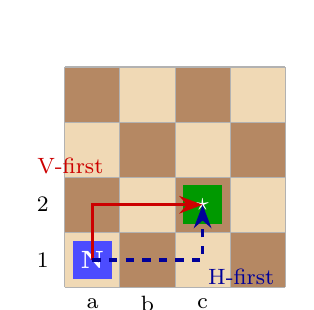
\begin{tikzpicture}[scale=0.7]
    % Draw grid
    \foreach \r in {0,...,3} {
        \foreach \c in {0,...,3} {
            \pgfmathparse{mod(\r+\c,2)==0 ? "squarelight" : "squaredark"}
            \edef\col{\pgfmathresult}
            \fill[\col] (\c,\r) rectangle ++(1,1);
        }
    }
    \draw[step=1cm, black!30, thin] (0,0) grid (4,4);

    % Source at (0,0) -> display bottom-left
    \fill[blue!70]   (0.15,0.15) rectangle ++(0.7,0.7);
    \node[white, font=\bfseries\small] at (0.5, 0.5) {N};

    % Destination: knight move (+1 row, +2 col) in grid coords = display col+2, row+1
    \fill[green!60!black] (2.15,1.15) rectangle ++(0.7,0.7);
    \node[white, font=\bfseries\small] at (2.5, 1.5) {$\star$};

    % Vertical-first path: (0,0)->(1,0)->(1,1)->(1,2)
    \draw[-Stealth, red!80!black, very thick] (0.5,0.5) -- (0.5,1.5) -- (1.5,1.5) -- (2.5,1.5);
    \node[red!80!black, font=\footnotesize] at (0.1, 2.2) {V-first};

    % Horizontal-first path: (0,0)->(0,1)->(0,2)->(1,2)
    \draw[-Stealth, blue!60!black, very thick, dashed]
        (0.5,0.5) -- (1.5,0.5) -- (2.5,0.5) -- (2.5,1.5);
    \node[blue!60!black, font=\footnotesize] at (3.2, 0.2) {H-first};

    % Labels
    \node[font=\footnotesize] at (0.5, -0.3) {a};
    \node[font=\footnotesize] at (1.5, -0.3) {b};
    \node[font=\footnotesize] at (2.5, -0.3) {c};
    \node[font=\footnotesize] at (-0.4, 0.5) {1};
    \node[font=\footnotesize] at (-0.4, 1.5) {2};
\end{tikzpicture}
\end{center}

\subsection{Bishop}

\function{generateBishopPath(const BoardCoord\& from, const BoardCoord\& to)}{Function}{\texttt{from}, \texttt{to} -- source and destination coordinates}{\texttt{std::vector<Path>} with exactly one path}

Delegates to \texttt{generateDiagonalPath}, producing a single path that steps one square diagonally at a time toward the destination.

\subsection{Rook}

\function{generateRookPath(const BoardCoord\& from, const BoardCoord\& to)}{Function}{\texttt{from}, \texttt{to} -- source and destination coordinates}{\texttt{std::vector<Path>} with exactly one path}

Delegates to \texttt{generateOrthogonalPath}, stepping either horizontally or vertically depending on the direction of the move.

\subsection{Queen}

\function{generateQueenPath(const BoardCoord\& from, const BoardCoord\& to)}{Function}{\texttt{from}, \texttt{to} -- source and destination coordinates}{\texttt{std::vector<Path>} with exactly one path}

Selects diagonal movement when \texttt{|rowDiff| == |colDiff|}, orthogonal movement otherwise. Returns a single path.

\subsection{King}

\function{generateKingPath(const BoardCoord\& from, const BoardCoord\& to)}{Function}{\texttt{from}, \texttt{to} -- source and destination coordinates}{\texttt{std::vector<Path>} with exactly one path containing only the destination square}

King moves are always a single square. The path contains only the destination, so the gantry moves directly without intermediate steps.

\section{Primitive Path Helpers}

Two low-level helpers are shared by multiple generators:

\function{generateDiagonalPath(const BoardCoord\& from, const BoardCoord\& to)}{Function}{\texttt{from}, \texttt{to} -- source and destination}{\texttt{Path}}

Steps one square per iteration with equal row and column increments (signs determined by the direction of travel) until the destination is reached. All intermediate squares plus the destination are included.

\function{generateOrthogonalPath(const BoardCoord\& from, const BoardCoord\& to)}{Function}{\texttt{from}, \texttt{to} -- source and destination}{\texttt{Path}}

Steps one square per iteration along either a row or a column (one of the step values is always zero). Implementation is identical to \texttt{generateDiagonalPath}; the distinction lies in what \texttt{from}/\texttt{to} pairs are passed by the callers.

\section{Path Selection}

\function{selectBestPath(const PhysicalBoard\& board, const std::vector<Path>\& paths)}{Function}{\texttt{board} -- current physical board state; \texttt{paths} -- candidate paths}{\texttt{Path} -- the path with the fewest blocking pieces}

Iterates over all candidate paths, calling \texttt{findBlockers} on each, and returns the path whose blocker count is minimal. If two paths tie, the earlier one in the vector wins. If the input vector is empty, returns an empty \texttt{Path}.

%==============================================================================
\chapter{Blocker Detection and Relocation}
%==============================================================================

\section{Blocker Detection}

\function{findBlockers(const PhysicalBoard\& board, const Path\& path)}{Function}{\texttt{board} -- current occupancy; \texttt{path} -- the path to inspect}{\texttt{std::vector<BoardCoord>} -- occupied intermediate squares}

Scans every square in \texttt{path} \emph{except} the destination and returns all that are occupied. The destination is excluded because captures are handled separately by the gantry controller (the captured piece is removed before the primary move begins).

\section{Parking Spot Selection}

When a blocker must be moved temporarily, it needs to be placed on an empty square that is not on the primary piece's path. The parking spot finder uses BFS expanding outward from the blocker's position to find the nearest such square.

\function{findParkingSpot(const PhysicalBoard\& board, const BoardCoord\& blockerPos, const std::set<BoardCoord>\& excludeSquares)}{Function}{\texttt{board} -- current occupancy; \texttt{blockerPos} -- the blocker's current position; \texttt{excludeSquares} -- squares that must not be used}{\texttt{BoardCoord} -- nearest valid parking spot, or \texttt{BoardCoord(-1,-1)} on failure}

The BFS explores the 8-connected neighbourhood of each visited square. A candidate square is accepted when it is empty and not in \texttt{excludeSquares}. The \texttt{excludeSquares} set is pre-populated with every square on the primary piece's path, ensuring that parked pieces do not block the main move.

\section{Recursive Blocker Relocation}

\begin{lstlisting}[language=C++, caption={Blocker relocation signature (internal)}]
static bool planBlockerRelocation(
    PhysicalBoard&              board,
    const BoardCoord&           blockerPos,
    std::set<BoardCoord>&       excludeSquares,
    std::vector<RelocationPlan>& relocations,
    int                         depth);
\end{lstlisting}

This internal function handles the case where the path to the parking spot is itself blocked. The algorithm proceeds as follows:

\begin{enumerate}
    \item Find a parking spot for the blocker via \texttt{findParkingSpot}.
    \item Attempt to find a clear path to the parking spot using A* (\texttt{findClearPath}).
    \item If a clear path exists, record the \texttt{RelocationPlan} and update the board state. Done.
    \item If no clear path exists, identify the pieces blocking the route to the parking spot using a secondary BFS.
    \item Recursively call \texttt{planBlockerRelocation} for each of those secondary blockers (depth-first).
    \item After recursive relocations, retry A* to the parking spot.
    \item If still blocked, try up to five alternative parking spots.
    \item Return \texttt{false} if no solution is found.
\end{enumerate}

A maximum recursion depth of 16 is enforced to prevent infinite loops in degenerate board configurations.

\begin{algorithm}
\caption{Recursive Blocker Relocation}
\begin{algorithmic}[1]
\Procedure{planBlockerRelocation}{board, blockerPos, excludeSquares, relocations, depth}
    \If{depth $>$ MAX\_DEPTH (16)}
        \Return false
    \EndIf
    \State parkingSpot $\gets$ \Call{findParkingSpot}{board, blockerPos, excludeSquares}
    \If{parkingSpot is invalid}
        \Return false
    \EndIf
    \State path $\gets$ \Call{findClearPath}{board, blockerPos, parkingSpot}
    \If{path is not empty}
        \State record relocation, update board
        \Return true
    \EndIf
    \State pathBlockers $\gets$ BFS to find blockers between blockerPos and parkingSpot
    \ForAll{pb $\in$ pathBlockers}
        \If{board.isOccupied(pb)}
            \If{not \Call{planBlockerRelocation}{board, pb, excludeSquares, relocations, depth+1}}
                \Return false
            \EndIf
        \EndIf
    \EndFor
    \State path $\gets$ \Call{findClearPath}{board, blockerPos, parkingSpot}
    \If{path is empty}
        \State try up to 5 alternative parking spots
    \EndIf
    \If{path is still empty}
        \Return false
    \EndIf
    \State record relocation, update board
    \Return true
\EndProcedure
\end{algorithmic}
\end{algorithm}

%==============================================================================
\chapter{A* Pathfinding}
%==============================================================================

\section{Overview}

A* pathfinding is used exclusively for routing blocker pieces to their parking spots. Unlike primary piece paths (which follow chess movement rules), blocker paths must avoid all occupied squares and find the shortest physically traversable route.

\function{findClearPath(const PhysicalBoard\& board, const BoardCoord\& from, const BoardCoord\& to)}{Function}{\texttt{board} -- current occupancy; \texttt{from} -- start; \texttt{to} -- goal}{\texttt{Path} -- shortest clear path, or empty path if none exists}

\section{Algorithm Details}

The implementation uses a standard A* search over the 8-connected grid:

\begin{itemize}
    \item \textbf{Open set}: \texttt{std::priority\_queue} (min-heap) of \texttt{AStarNode} values keyed on $f = g + h$.
    \item \textbf{Heuristic} $h$: Chebyshev distance (maximum of $|\Delta\text{row}|$ and $|\Delta\text{col}|$), which is admissible because the gantry can move diagonally and each step costs 1.
    \item \textbf{Edge cost}: Uniform cost of 1 per step regardless of direction.
    \item \textbf{Obstacle avoidance}: Occupied squares are skipped, except for the goal square (which may be occupied by the piece being relocated there).
    \item \textbf{Path reconstruction}: Follows \texttt{cameFrom} pointers from goal back to start, then reverses.
\end{itemize}

\begin{lstlisting}[language=C++, caption={AStarNode definition}]
struct AStarNode {
    BoardCoord coord;
    int        fScore;   // g + h

    bool operator>(const AStarNode& other) const {
        return fScore > other.fScore;
    }
};
\end{lstlisting}

\section{Distance Metrics}

Two distance metrics are defined for use in heuristics and path evaluation:

\function{chebyshevDistance(const BoardCoord\& from, const BoardCoord\& to)}{Function}{\texttt{from}, \texttt{to} -- two squares}{\texttt{int} -- $\max(|\Delta r|, |\Delta c|)$}

The Chebyshev (chessboard) distance is the minimum number of king moves needed. It is the A* heuristic because the gantry can step diagonally.

\function{manhattanDistance(const BoardCoord\& from, const BoardCoord\& to)}{Function}{\texttt{from}, \texttt{to} -- two squares}{\texttt{int} -- $|\Delta r| + |\Delta c|$}

Manhattan distance counts only orthogonal steps. Available for use in contexts where diagonal travel is not permitted.

%==============================================================================
\chapter{Move Planning}
%==============================================================================

\section{planMove}

\function{planMove(PhysicalBoard\& board, const PhysicalMove\& move)}{Function}{\texttt{board} -- current physical board state (will be read but not permanently modified); \texttt{move} -- the physical chess move to plan}{\texttt{MovePlan} -- complete execution plan}

This is the primary entry point for the board interpreter. It orchestrates all sub-systems to produce the complete \texttt{MovePlan}. The board parameter is passed by reference to allow temporary mutation during planning via a local copy; the original is not modified.

\section{Planning Algorithm}

\begin{enumerate}
    \item \textbf{Generate candidate paths} for the primary piece by calling \texttt{generatePath(move)}.
    \item \textbf{Select the best path} using \texttt{selectBestPath}, which minimises the number of blockers.
    \item \textbf{Identify all blockers} on the chosen path using \texttt{findBlockers}. Intermediate squares only; the destination is excluded.
    \item \textbf{Build the exclusion set} containing every square on the primary path and the primary piece's source square.
    \item \textbf{Copy the board} into \texttt{tempBoard}. All subsequent mutations happen on this copy.
    \item \textbf{Plan blocker relocations}: for each blocker call \texttt{planBlockerRelocation}, which recursively handles secondary blockers and appends \texttt{RelocationPlan} entries to \texttt{plan.relocations}.
    \item \textbf{Apply the primary move} to \texttt{tempBoard} so the restored post-move board state is available for restoration path planning.
    \item \textbf{Plan restorations}: iterate over \texttt{relocations} in reverse order (LIFO). For each relocation, call \texttt{findClearPath} from the parking spot back to the piece's original square. During execution, the gantry follows this restoration path when it exists; if no clear path exists, the path is left empty and the gantry controller falls back to a direct move.
    \item \textbf{Mark the plan valid} and return.
\end{enumerate}

\section{Error Handling}

\texttt{MovePlan.isValid} is set to \texttt{false} and \texttt{MovePlan.errorMessage} is populated in the following failure cases:

\begin{table}[h]
\centering
\begin{tabular}{ll}
\toprule
\textbf{Condition} & \textbf{Error Message} \\
\midrule
No paths generated for piece type & \texttt{"No paths generated for move"} \\
\texttt{selectBestPath} returns empty & \texttt{"No valid path found"} \\
Blocker cannot be relocated & \texttt{"Cannot relocate blocker (position too constrained)"} \\
\bottomrule
\end{tabular}
\caption{MovePlan failure modes}
\end{table}

\warningbox{If \texttt{planMove} returns an invalid plan, the gantry controller must not attempt to execute it. The game controller layer is responsible for checking \texttt{MovePlan.isValid} before dispatching commands.}

%==============================================================================
\chapter{Utility Functions and Bitboard Helpers}
%==============================================================================

\section{Neighbour Enumeration}

\function{getNeighbors(const BoardCoord\& pos)}{Function}{\texttt{pos} -- a board coordinate}{\texttt{std::vector<BoardCoord>} -- up to 8 valid neighbouring squares}

Returns all 8-connected neighbours of \texttt{pos} that lie within the board boundary. Used by both the BFS parking-spot finder and the A* pathfinder. Corner squares yield 3 neighbours, edge squares yield 5, and interior squares yield 8.

\section{Inline Helper}

\function{sign(int val)}{Inline Function}{\texttt{val} -- any integer}{\texttt{int} -- $-1$, $0$, or $1$}

Returns the arithmetic sign of \texttt{val}. Used extensively in path generation to compute step directions along rows and columns.

\section{Bitboard Utilities}

These are standalone utility functions operating on \texttt{Bitboard} (\texttt{uint64\_t}) values. They mirror the conventions of the Kirin engine's own bitboard layer so that occupancy information received from the engine can be consumed directly.

\begin{table}[h]
\centering
\begin{tabular}{lll}
\toprule
\textbf{Function} & \textbf{Signature} & \textbf{Description} \\
\midrule
\texttt{bb\_setBit}   & \texttt{(Bitboard\&, int)} & Set bit at square index \\
\texttt{bb\_clearBit} & \texttt{(Bitboard\&, int)} & Clear bit at square index \\
\texttt{bb\_getBit}   & \texttt{(Bitboard, int) -> bool} & Test bit at square index \\
\texttt{bb\_countBits}& \texttt{(Bitboard) -> int} & Popcount via Kernighan's method \\
\texttt{bb\_getLSB}   & \texttt{(Bitboard) -> int} & Index of least significant set bit; $-1$ if zero \\
\bottomrule
\end{tabular}
\caption{Bitboard utility functions}
\end{table}

\texttt{bb\_setBit}, \texttt{bb\_clearBit}, and \texttt{bb\_getBit} are declared \texttt{inline} in the header for maximum performance. \texttt{bb\_countBits} uses the bit-manipulation trick \texttt{bb \&= bb - 1} to clear the lowest set bit on each iteration.

\section{Position Parsing}

\function{parseBoardPosition(const char* pieces)}{Function}{\texttt{pieces} -- space-separated list of piece-square tokens (e.g. \texttt{"Pe2 Nd5 Rb1"})}{\texttt{Bitboard} -- occupancy bitboard}

Converts a human-readable piece list into an occupancy bitboard for testing or manual board setup. Each token consists of an optional piece-type letter followed by a two-character square name. The function is tolerant of extra whitespace and skips malformed tokens.

%==============================================================================
\chapter{Debug Functions}
%==============================================================================

\section{printPath}

\function{printPath(const Path\& path)}{Function}{\texttt{path} -- the path to display}{void}

Prints the sequence of squares in a path to \texttt{stdout} using FEN algebraic notation, e.g.:

\begin{lstlisting}
Path (4 squares): e4 e5 e6 e7
\end{lstlisting}

\section{printMovePlan}

\function{printMovePlan(const MovePlan\& plan)}{Function}{\texttt{plan} -- the move plan to display}{void}

Prints a complete human-readable summary of a \texttt{MovePlan}. For invalid plans it displays the error message. For valid plans it prints the primary move, primary path, each relocation with its path, and each restoration with its path (or a note if no path was found). Example output:

\begin{lstlisting}
=== Move Plan ===
Primary Move: e2 -> e4
Primary Path: Path (2 squares): e3 e4

Relocations (1):
  1. d3 -> a3: Path (3 squares): c3 b3 a3

Restorations (1):
  1. a3 -> d3: Path (3 squares): b3 c3 d3
=================
\end{lstlisting}

%==============================================================================
\chapter{Testing}
%==============================================================================

\section{Test Coverage}

The board interpreter test suite is located in \texttt{board\_interpreter\_test.cpp}. It covers:

\begin{itemize}
    \item \textbf{Coordinate conversion}: round-trip tests for \texttt{fromFEN}/\texttt{toFEN} and \texttt{toSquareIndex}/\texttt{fromSquareIndex}.
    \item \textbf{Path generation}: correctness tests for all six piece types including edge cases (pawn double move, knight at board corners, king move).
    \item \textbf{Blocker detection}: tests with zero, one, and multiple blockers at various positions on a path.
    \item \textbf{Parking spot finding}: empty board, fully occupied board, and paths where all nearby squares are excluded.
    \item \textbf{A* pathfinding}: clear board, simple obstacles, and constrained configurations.
    \item \textbf{Move planning}: end-to-end tests for moves with no blockers, single blockers, multiple blockers, and captures.
\end{itemize}

Additionally, \texttt{captured\_piece\_test.cpp} validates the interaction between the board interpreter and the gantry controller for capture moves, ensuring the captured piece is handled before the primary move path is traversed.

\section{Running Tests}

Build and run the test suite with CMake:

\begin{lstlisting}[language=bash]
cd build
cmake .. -DBUILD_TESTS=ON
make
ctest --output-on-failure
\end{lstlisting}

%==============================================================================
\chapter{Integration Guide}
%==============================================================================

\section{Typical Usage Pattern}

The following code illustrates the typical call sequence for executing an engine move:

\begin{lstlisting}[language=C++, caption={Typical board interpreter usage}]
#include "board_interpreter.h"

// 1. Receive occupancy from the engine
Bitboard occupancy = engine.getOccupancyBitboard();

// 2. Set up the physical board
PhysicalBoard board;
board.setOccupancy(occupancy);

// 3. Build the physical move descriptor
PhysicalMove move;
move.from      = BoardCoord::fromFEN("e2");
move.to        = BoardCoord::fromFEN("e4");
move.pieceType = PAWN;
move.isCapture = false;

// 4. Plan the move
MovePlan plan = planMove(board, move);

// 5. Check validity and dispatch
if (!plan.isValid) {
    fprintf(stderr, "Board interpreter error: %s\n", plan.errorMessage);
    return;
}

// 6. Hand off to gantry controller
gantryController.executePlan(plan);
\end{lstlisting}

\section{Capture Moves}

For capture moves, set \texttt{PhysicalMove::isCapture = true}. The board interpreter itself does not remove the captured piece from the occupancy bitboard — it treats the destination square as empty for path-planning purposes (by excluding it from blocker detection). The gantry controller is responsible for lifting the captured piece off the board before the primary move begins, using the off-board staging area defined in the gantry configuration.

\section{Special Chess Moves}

\subsection{Castling}

Castling must be decomposed into two \texttt{PhysicalMove} operations by the game controller before being passed to the board interpreter:

\begin{enumerate}[noitemsep]
    \item King move: e.g. \texttt{e1 -> g1}
    \item Rook move: e.g. \texttt{h1 -> f1}
\end{enumerate}

Each is planned independently and the resulting \texttt{MovePlan} values are executed in sequence. The game controller layer in \texttt{game\_controller.cpp} is responsible for this decomposition.

\subsection{En Passant}

En passant is handled similarly: the pawn's physical move is planned normally, and the capture of the opponent's pawn (which sits on a different square from the destination) is an additional operation the game controller schedules separately.

\subsection{Promotion}

Promotion is transparent to the board interpreter. The pawn moves to the back rank and the piece identity change is an engine-level concern; the physical gantry simply moves the pawn and the game controller then coordinates any physical piece swap with the captured-piece area.

%==============================================================================
\appendix
\chapter{Glossary}
%==============================================================================

\begin{description}
    \item[A*] An informed graph search algorithm that finds the shortest path using a heuristic to guide exploration.
    \item[BFS] Breadth-First Search; explores all nodes at a given distance before proceeding further. Used here for parking-spot selection.
    \item[Bitboard] A 64-bit integer where each bit represents one square of the chess board. Bit set = square occupied.
    \item[Blocker] A piece that sits on an intermediate square of another piece's intended movement path.
    \item[BoardCoord] The \texttt{(row, col)} struct representing a physical square on the board.
    \item[Chebyshev Distance] The maximum of $|\Delta r|$ and $|\Delta c|$ between two squares; equals the minimum number of king moves.
    \item[FEN] Forsyth-Edwards Notation; used here to identify squares via two-character algebraic names (e.g.\ \texttt{e4}).
    \item[Gantry] The motorised XY carriage beneath the board that moves a magnet to drag pieces.
    \item[Manhattan Distance] The sum $|\Delta r| + |\Delta c|$; minimum steps if only orthogonal movement is allowed.
    \item[MovePlan] The complete, ordered execution plan for one chess move on the physical board.
    \item[Parking Spot] A temporary empty square to which a blocking piece is relocated while the primary move is executed.
    \item[Path] An ordered sequence of \texttt{BoardCoord} values (not including source) that the gantry head traverses.
    \item[PhysicalBoard] The occupancy-tracking class used during move planning; mutated on a temporary copy.
    \item[PhysicalMove] A simple descriptor of a piece movement: source, destination, piece type, and capture flag.
    \item[RelocationPlan] A plan to temporarily move a single blocker to a parking spot, including the route.
    \item[Restoration] The return of a temporarily parked piece to its original square after the primary move completes.
\end{description}

%==============================================================================
\chapter{References}
%==============================================================================

\begin{itemize}
    \item Kirin Chess Engine source: \texttt{engine.h}, \texttt{position.h}, \texttt{bitboard.h}
    \item Gantry Controller interface: \texttt{gantry\_controller.h}
    \item Game Controller integration: \texttt{game\_controller.h}
    \item A* Search Algorithm: \url{https://en.wikipedia.org/wiki/A*_search_algorithm}
    \item Chebyshev distance in chess contexts: \url{https://www.chessprogramming.org/Distance}
    \item Kernighan's bit-counting method: Brian W. Kernighan and Dennis M. Ritchie, \textit{The C Programming Language}, 2nd ed., exercise 2-9.
\end{itemize}

%%%%%%%%%%%%%%%%%%%%%%%%%%%%%%%%%%%%%%%%%%%%%%%%%%%%%%%%%%%%%%%%%%%%%%%%%%%%%%%
\end{document}
%%%%%%%%%%%%%%%%%%%%%%%%%%%%%%%%%%%%%%%%%%%%%%%%%%%%%%%%%%%%%%%%%%%%%%%%%%%%%%%
